\chapter{Background\label{cha:background}}

In this chapter, we discuss traditional artificial intelligence in the context of search the algorithms we used, what some other similar methods exist as well as the field in general. We allocate a large portion of the section to Breakthrough as that will be the testbed for future sections. We discuss the different classes of machine learning as well as discuss neural networks in more depht.

\section{Environments}
\label{sec:environments}

When researching Artificial Intelligence it is important to select an environment that is a suitable abstraction for the task at hand. Environments vary significantly and can be identified by their characteristic. The characteristics that are generally used to describe environments can be seen in Table~\ref{tab:env_characteristics}. This categorization of environments is described in the book Artificial Intelligence by Norvig \& Russell. \cite{Russell:AIModern}

\begin{table}[ht]
  \centering
  \begin{tabular}{|c|c|p{6cm}|}
    \hline
    \textbf{characteristic} & \textbf{Values}              & \textbf{Description}                                                                 \\
    \hline
    Observable              & Fully, Partially             & How much of the environment can your agent percieve.                                 \\
    \hline
    Agents                  & Single, Multi                & Are there multiple agents playing in the environment.                                \\
    \hline
    Deterministic           & Deterministic, Stochastic    & Do the actions your agent do deterministicly impact the environment.                 \\
    \hline
    Episodic                & Sequential, Episodic         & Are actions episodic or sequential.                                                  \\
    \hline
    Static                  & Static, Semi-Static, Dynamic & Does the environment without agent input, or does it wait until agents take actions. \\
    \hline
    Discrete                & Discrete, Continuous         & Is your environment discrete w.r.t actions.                                          \\
    \hline
  \end{tabular}
  \caption{Characteristics of environments}
  \label{tab:env_characteristics}
\end{table}

Categorizing environments like this gives you the power to find an environment in which a method works and know it can be applied to different environments with the same characteristics. Additionally, it allowes us to talk about agents in the context of environments as the entities that act within the environment.

\section{Game Environment}

With classical Artificial Intelligence Game Environments are commonly used to validate a method, game environments can be games like Tic-Tac-Toe, Breakthrough, and driving simulators. Game environments are a suitable place to apply AI as they serve an important function as an abstraction of the real world, for instance, a self-driving car agent who is verified to avoid driving into walls in a simulation is possibly safer than one who is not.

\section{Breakthrough}

The game breakthrough is a simplified version of chess, the game is set up on a $MxN$ board with cells like in chess, and each player starts with two rows of pawns at either end. The objective of the game is for a player to move one of their pawns to the opposite end of the board. A player wins if either they have reached the opposite end of the board or have captured all of his opponents' pawns. The pawns differ from chess pawns in such a way that they can not move two squares on the first move and, they can move diagonally as well as forward, this leads to the game being impossible to draw as pieces are always able to move. An example of an initial board in breakthrough can be seen in Figure~\ref{fig:initbtboard}

\begin{figure}[]
  \centering

  \breakthrough{8/8/pppppp2/pppppp2/8/8/PPPPPP2/PPPPPP2 w - - 0 1}

  \caption{Initial breakthrough board}
  \label{fig:initbtboard}
\end{figure}


\begin{table}[ht]
  \centering
  \begin{tabular}{|c|c|}\hline
    \textbf{Characteristic} & \textbf{Value} \\\hline
    Observable              & Fully          \\
    Agents                  & Multi          \\
    Deterministic           & Deterministic  \\
    Episodic                & Sequential     \\
    Static                  & Static         \\
    Discrete                & Discrete       \\\hline
  \end{tabular}
  \caption{Categorization of Breakthrough}
  \label{tab:breakthrough_cat}
\end{table}

Categorizing Breakthrough with the characteristics described in Section~\ref{sec:environments}. We end up with the description shown in Table~\ref{tab:breakthrough_cat}. These characteristics are identical to that of Tic-Tac-Toe, and Chess. This categorization is the most common in board games where two-player compete.

\subsection{Heuristics of Breakthrough}

To evaluate the game of Breakthrough we can consider many heuristics (higher-level concepts) for instance a very simple heuristic would be a players Material Advantage. Material Advantage is the amount of pieces the player has minus the amount of pieces the opponent has. This heuristics gives us some insight into how well the game is progressing, but obviously, there are cases where this doesn't tell us much, as in cases when your opponent has a single piece left that is on the row immediately before the row needed for him to win. No matter how many pieces you have left, this state is bad for you if you're not able to capture that piece. An example of such a state can be seen in Figure~\ref{fig:bt_h1_bad}.

\begin{figure}[]
  \centering
  \breakthrough{8/8/pppp4/pp3P2/2p5/8/8/8 w - - 0 1}
  \caption{Breakthrough board where Material Advantage doesn't work well}
  \label{fig:bt_h1_bad}
\end{figure}

A different heuristic would be the distance of your most advanced pawn minus your opponents most advanced pawn, this heuristic could give you insight into how close you are to winning the game or how close your opponent is. As a higher-level concept, we can call this concept your aggressiveness, as it closely resembles how aggressive you are going for in for the win. Generally, in Breakthrough, it is favorable to move your whole team as a unit and play more defensively, and additional heuristics for Breakthrough will be discussed in detail later in this research.

\section{State-Space Search}

Traditionally methods for playing games were searching through the environment using a heuristic to guide the search. A simple way of doing a heuristic-based search would be to give all states a $0$ as a score and give states where you win a positive score. We say that that search algorithm is not guided, and the algorithm will probably have to evaluate every state in the state-space. This method of searching is generally extremely inefficient as the state-spaces of game environments are often extremely large, and sometimes infinite. For instance, an upper-bound estimate of the state-space for breakthrough is $3^{(M-1)*(N-1)}+2*N$ where $M$ is the height of the board $N$ is the width of the board. The $3^{(M-1)*(N-1)}$ represents each position of the board having either a white, or black piece, or being empty. So for a small board, $5x4$ the upper-bound estimation of the state-space is $531,449$ states.

This is why a good heuristic is very valuable because we can disregard all following states that result from doing a move some in a previous state as they will only lead to worse outcomes.

The algorithms that are used in traditional state-space searches are for instance Depth-first search (DFS), Breadth-first Search (BFS), Alpha-Beta Pruning Search (AB-Search), and Monte-Carlo Tree Search (MCTS).

More modernly, these search methods have been amplified by Machine Learning, in such a way that we do not need to figure out a good heuristic for a given state, but rather, we apply a machine learning model to learn a function that takes in a state and returns an evaluation of that state.\cite{neuralnetworksgames:michulke} This can lead to a significant time reduction as we do not need to simulate a whole game from a state to receive its evaluation we rather receive the evaluation from the model.

\subsection{Monte-Carlo Tree Search}

\label{sec:mcts}

In the algorithm Monte-Carlo Tree Search, there is an agent within some environment. Where each node in the environment represents a state-action pair of the environment, by state-action pair what is meant it is some state and the action that brought the agent to that state. This pair should be unique within the environment.

MCTS is a method of exploring an environment in a randomized manner (Monte Carlo is the term implying randomness). In MCTS there are four stages. Selection, Expansion, Simulation, and Back-propagation. They happen sequentially and repeatedly. MCTS is initialized with a tree consisting of the unexpanded initial state of the environment.

In MCTS there is a tree representing the game-environment. This tree consists of nodes $n_i$ where $i$ represents the point in time of the node, for example, $N_0$ in chess is the initial position and $N_x$ is some position in the middle of the game and $N_e$ is one of the states representing a position where there is either a draw or one player has won the match. Each of the nodes has $4$ values, $s$, $a$, $Q$, and $N$. These values represent these items, $s$ is the state of the environment, $a$ is the action that brought the previous node $n_{i-1}$ to node $n_i$, $Q$ is the average reward from running the MCTS algorithm from this node, and $N$ the number of times the MCTS algorithm has visited this node. The values $s$ and $a$ uniquely identify a position in the environment and are often called state-action pairs.

The MCTS algorithms four phases
\begin{enumerate}
  \item Selection
  \item Expansion
  \item Simulation/Rollout
  \item Backpropagation
\end{enumerate}


\begin{equation} \label{UCT_formula}
  \text{Child UCT value} = \frac{Q_{(s',a')}}{N_{(s',a')}} + c_{uct} * \frac{\sqrt{log(N_{(s,a)})}}{N_{(s',a')}}
\end{equation}

\subsection*{Selection}
During the selection phase, a node $(s,a)$ within the tree which has not yet been expanded is found.
This process uses Upper Confidence Bound on Trees (UCT) to find that node $(s,a)$, the formula is described in Equation \ref{UCT_formula}. For a parent node $(s,a)$
(initially the root of the tree) we select the child with the highest UCT value. Repeatedly until an unexpanded
node is found. This process is done to balance the amount of exploration vs exploitation of nodes in the
tree.

\subsection*{Expansion}
Then the expansion phase expands the node generating all of $(s,a)$'s children, $(s',a')$ are generated by applying all actions $a'$ in $(s,a)$.

\subsection*{Rollout}
Next during rollout, actions from $(s,a)$ are randomly selected to move to $(s',a')$, then repeated to go to $(s'',a'')$, until a terminal node within the environment is reached. By terminal, we mean a state in which the game is finished. A terminal node in MCTS can generally return any value, but in the context of this paper, we only return (+1 white wins, or -1 black wins).


\subsection*{Backpropagation}
The result from the terminal node is then propagated up through the path taken by selection $(s,a)$ up
to the root of the tree, updating the $Q_{(s,a)}$ values of each node $(s,a)$.

When training a neural network the UCT formula is modified slightly to prefer selecting nodes
that the neural network values highly by introducing a second scalar to the formula $f((s,a)) = (p,v)$, where $f$ is the neural network, $p$ is the policy vector returned by the neural network and $v$ is the predicted value from the neural network. The resulting formula is described in Equation \ref{PUCT_formula}, and is called PUCT. Secondly, the backpropagation process
is modified to instead of doing rollout/simulation to receive a reward the predicted value $v$ from the neural network is used instead.

\begin{equation} \label{PUCT_formula}
  \text{Child PUCT value} = \frac{Q_{(s',a')}}{N_{(s',a')}} + c_{uct} * p_{(s,a)} * \frac{\sqrt{log(N_{(s,a)})}}{N_{(s',a')}}
\end{equation}

\section{Machine Learning}

Machine Learning (ML) is a research field in which machines apply statistical functions on data to achieve a correct output, by \textit{correct} we mean the corresponding result which we expect. Generally, this a repetitive process where we look at examples of the data, and the algorithm progressively gets closer to the underlying function of the data it is fed. This process is therefore similar to trial and error for humans. ML is a sub-field of Artificial Intelligence. ML algorithms come in the form of two classes \textit{Classification}, where the algorithm should find a class representing the data it is given, and \textit{Regression} where the algorithm should find an underlying continuous numerical function and will return a numerical value representing the input.

Typically ML can be viewed in three different groups, Supervised Learning, Reinforcement Learning (RL), and Unsupervised Learning. Where in Supervised Learning, the algorithm is given data examples and their corresponding outcome. For example, a supervised learning algorithm could be provided with data regarding the weather and the corresponding temperature, the algorithm should then find a pattern within the weather data and find the continuous function represented by the data. This would then be an example of a regression task. Flipping thing example around, if the algorithm would just be provided the temperature and it should tell us whether it is sunny outside or not, that would be a classification task.

In RL the algorithm is given only some input, and then the algorithm tries some outcome generally actions in some environment. Then over an episode~\footnote{a series of outcomes / a timespan} once the episode is finished some reward is given. The algorithm will then learn whether the actions were good actions from the reward. Examples of this are agents playing a game like Flappy Bird, where the data they are given is the state of the game, and they try to either jump or not jump.

%Machine learning (ML) focuses on the using of data and a corresponding outcome w.r.t that data to 
%extrapolate some underlying function of that data. Examples of how we use machine learning is for instance the ability to predicting the 
%rise and fall of some stock, predicting what the weather will be in a week, and whether an image 
%is an image of a dog or a cat. Many data structures and algorithms are used to achieve this 
%goal, but recently the field of ANN/DNN's has been the standard for achieving the best
%results.

%As a general notion we can split machine learning into three different sects those are Supervised Learning, Reinforcement Learning, and Unsupervised Learning.

\subsection{Supervised Learning}

In supervised learning, the data and their corresponding outcomes are already available to us. Examples of the data we can use in supervised learning would be labeled images.

\subsection{Reinforcement Learning}

Reinforcement Learning is where a model learns from experience. That is, the notion of input/output values changes, the model uses itself to generate input values by acting in an environment. The environment then returns some result, that could be losing in a game, making a correct prediction, or any number of outcomes. The result is then propagated through the model allowing it to improve with this new information.
% When doing moving it's parameters in the direction of the recieved output
% from the environment.

Many algorithms are popular in reinforcement learning, for instance Q-learning(CITE ME), CARLA (CITE ME),
and many others.

\subsection{Neural Networks}

Neural networks (NN) are popular methods within a sub-field of ML which is called Deep Learning (DL).
NN's are created to resemble how the human brain functions. In the brain, we have neurons which when they get a signal they apply some function to them and if the resulting signal is high enough, they fire to the next neuron. This is how it is done in the neural network model as well.
There we have neurons that when they get some input, generally a vector of numbers. The neuron takes the sum of that vector, weighs the sum by a constant, then applies a non-linear activation function to it. The result of doing this is then passed on to the next neuron. Until a final layer of neurons is reached. At that point, we have a value that the neural network corresponds to the input value. This value can be a binary classification (cat or dog image), a regression value (the value of a property), or any number of outputs. It can then be said that a neural network is doing a function approximation of the input to some value. $f_n ( w_n * f_{n-1} (w_{n-1} * \dots f_0(w_0*i))) = o$.

Neural networks are machine learning models that take in as input anything numerical and they apply continuous differentiable functions to that input s.t. they end with some output. This output is then compared to the expected output the difference between these outputs is called a loss. A loss is backpropagated through the neural network, and each function is derived to find its slope. We can then modify the weights of the neural network in the direction of the correct output. Leading to a function approximation of this function $f_{neuralnetwork}(X_{input}) = O_{expectedoutput}$

\section{Explainable Artificial Intelligence (XAI)}

The field of XAI research is still very far behind its counterpart AI research, within XAI two fields are the largest, those are Model Interpretability and Model Explainability.

\subsection{Model Interpretability}

Model Interpretability is the more common approach of XAI, as it is

\subsubsection{Saliency Maps}

Within XAI many methods have been developed to try to evaluate
ANN's, these methods are often referred as model interpretability methods.
In the field image recognition there has been a lot of work examining which
pixels of an image the model deems important. Arguably the most popular
method for this is Saliency Maps\cite{Koch:saliency}. There the pixel values the model
deems important are colored in s.t. a human can examine the image and get a
sense of what portions of the image are important to the model, an example of
a classification of a dog can be seen in Figure \ref{fig:dog_saliency}.

\begin{figure}[]
  \centering
  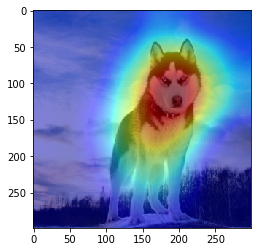
\includegraphics[width=.5\textwidth]{graphics/dog_saliency}
  \caption{Example of a models saliency map for an image of a dog}
  \label{fig:dog_saliency}
\end{figure}

While this method is understandable in the context of image recognition it
lacks severely when your input is not an image.

\subsubsection{Shapley Values}

Methods for explaining models that aren't image recognition models include
Shapley values, from the Lundberg \& Lee\cite{LundbergL:shapley}. There the input is examined against it's output, then iteratively
input values are selected to be fixed. Then the other input values are varied and
an average change in prediction is calculated. With this the shapley value can be
estimated for the fixed input value. This is done to examine which input values have
the strongest link to the output value. Shapley values on a dataset can give insights
on which input values the model deems important.

\subsubsection{Concept Activation Vectors}

A recent paper by Been Kim Et. al \cite{Keem:TCAV}, shows a method for examining
a neural network giving a much more human insight into a prediction. Using Concept
Activation Vectors (CAV) a directional derivative for a given input can be examined
with respect to some HLC's. For example, when a human looks at an image of an animal
and is supposed to decide whether the image is of a horse or a zebra, an intuitive
approach would be to check whether the animal has stipes, or the animal has both white and black colors.
That method of determining if a horse is a zebra could then be called a higher-level
concept, and if we're able to gather if a nerual network uses this strategy for prediction
we have a deeper understanding of its underlying structure. Leading to an explanation of
the result.

The construction of a CAV requires a method of labelling the values in your dataset with
the corresponding concept in order to create a simple binary classifier on the data points.

\subsection{Model Explainability}

Model explainability within the context of neural networks isn't possible today. Model
explainability referrs to firstly considering some input and output from a model. Then
afterwards the model is examined to determine exactly what led to the predicted output.
This concept is simple when we're working with Decision Trees. A decision tree is a tree
whose nodes are representative of an input value and at every node a branch is selected
based on the value of the input value. It is therefore easy to see how to examine the tree
to explain the output. We just follow the branches in the tree. That being said the branches
are created by algorithms like ID3 which construct branches based on the initial dataset used
to construct the tree, but again ID3 follows simple statistics and can be explained properly.


When we talk about neural networks this process is much more difficult, the underlying nodes
are generally in the thousands, the different layers of the neural network varies in the operations
it applies to the input value and such while travelling through the neural network the modified
value becomes far removed from the initial input value to the eyes of the reader. That being said,
while the possibility of completely monitoring the training process and completely monitoring the
evaluation process is truly possible it is not feasible. And secondly the process of seeing an
input and it's corresponding output will not be of any value if one were to consider the process
of prediction.

